\documentclass{standalone}
\usepackage{tikz}
\usepackage{amsmath}
\usetikzlibrary{angles, quotes, decorations.pathreplacing}

\begin{document}
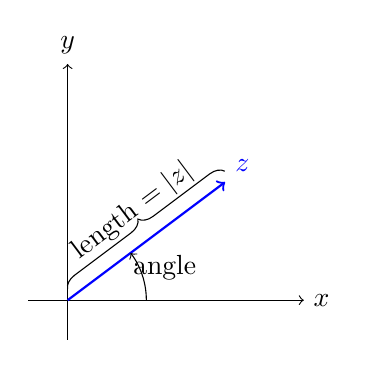
\begin{tikzpicture}[scale=1]

  % Axes
  \draw[->] (-0.5,0) -- (3,0) node[right] {$x$};
  \draw[->] (0,-0.5) -- (0,3) node[above] {$y$};

  % Vector z (blue)
  \draw[->, blue, thick] (0,0) -- (2,1.5) node[above right] {$z$};

  % Define coordinates for the angle
  \coordinate (O) at (0,0);
  \coordinate (A) at (1,0);
  \coordinate (B) at (2,1.5);

  % Angle (adjusted label position)
  \pic [draw, ->, "angle", angle eccentricity=1.3, angle radius=1cm] {angle = A--O--B};


  % Length (using a brace, placed ABOVE the vector)
  \draw [decorate,decoration={brace,amplitude=5pt},xshift=0pt,yshift=4pt]
    (0,0) -- (2,1.5) node [midway, above, sloped] {length $= |z|$};

\end{tikzpicture}
\end{document}